
\section{Experiments and Results} \label{sec:experimentsResults}

The performance of the torque and impedance controls have been assessed by experimental tests. 
The tests show how the torque controls behave in constant and varying desired torque tracking.
The first one is the transparency test in which the robot tries to keep the joint torque at zero Nm while the user is moving the exoskeleton.
The second test is the haptic rendering with a slanted flat surface with different simulated stiffness.
More details on each test are reported in the subsections below.
\par The implemented control laws (\ref{eq:JTCF1_control_law_uf_simple}), (\ref{JTFC2_control_law_final}) and (\ref{control_law_Kugi_2}) have been set using the model parameters. The proportional and derivative PD gains ($K_p$ and $K_d$) have been chosen to obtain a desired error dynamics, more in detail the form that guarantees the minimum ITAE index. Notice that the control laws (\ref{eq:JTCF1_control_law_uf_simple}) and (\ref{JTFC2_control_law_final}) have two degrees of freedom, i.e. $K_p$ and $K_d$ can be independently chosen, whereas the control law (\ref{control_law_Kugi_2}) exhibits a 1 degree of freedom, thus the two control gains are linked and they are calculated as a function of the desired inertia $J_{\theta}$.

%%%%%%%%%%%%%%%%%%%%%%%%%%%%%%%%%%%%%%%%%%%%%%%%%%%%%%%%%%%%%%%%%%%%%%%%%%%%%%%%%%%%%%%%%%%%%%%%%%%%%%%%%%%%%%%%%%%%
%%%%%%%%%%%%%%%%%%%%%%%%%%%%%%%%%%%%%%%%%%%%%%%%%%%%%%%%%%%%%%%%%%%%%%%%%%%%%%%%%%%%%%%%%%%%%%%%%%%%%%%%%%%%%%%%%%%%
\subsection{Transparency} \label{subsec:transparency}

For the transparency test, two kinds of trials have been done.
The first type of trial uses the JTFC1 control law described in the subsection \ref{subsec:JTFC1} in order to verify how much the dynamics compensations improve the desired torque tracking.
The second type of trials are useful to compare the three control laws and to understand how the terms of the control inputs are related to the desired torque tracking.
During the transparency tests the user has been linked with the exoskeleton in 2 points: the arm in order to transmit the shoulder movement, and the forearm in order to exchange the elbow movement.
\par In order to validate the interaction torque control and to evaluate the torque tracking performance, an additional force sensor has been mounted on the end-effector of the exoskeleton to measure the actual forces $\vects{F_h^*}$  applied by the user. 
As transparency index the measured end effector norm force and the reflected torques at the joints have been used.
The reflected torques at the joint are calculated as $\vects{\tau_s^*}=\vects{J^T F_h^*}$ and then compared to the interaction torques estimated by the optimal observer.

\subsubsection{How dynamic compensation affects the transparency} \label{subsubsec:compensationAndTransparency}

In order to understand how the dynamic compensation affects the transparency the scheme of figure \ref{fig:full state} has been implemented, that uses the JTFC1 control law plus the dynamics terms multiplied by $\alpha$, with $0 \leq \alpha \leq 1$.

The experimental results for torque tracking, with a desired torque $\vects{\tau_s^D=0}$, are shown for the second joint $J_2$ in \figurename \ \ref{fig:torque_validation}, that is the joint with the highest link inertia. A user has moved without constraints the exoskeleton, grabbing the force sensor mounted at the end effector. The control was set to follow his movement at zero-torque without (\figurename \ \ref{fig:torque_validation_nocomp}) and with (\figurename \ \ref{fig:torque_validation_comp}) dynamics compensation. 
\par The upper plots show the joint position (blue solid line) and acceleration (red dotted line), to demonstrate the movements were similar in both cases. The lower plots represent the interaction torques estimated by the observer (blue solid line) and measured by the force sensor (red dotted line). Even if the estimated torques are similar in both cases, with dynamics compensation the actual interaction forces are lower, demonstrating that torque tracking is more precise and the user has to compensate less for the links dynamics.

\begin{figure}[htb]
	\centering
	\subfigure[Without dynamics compensation]{ 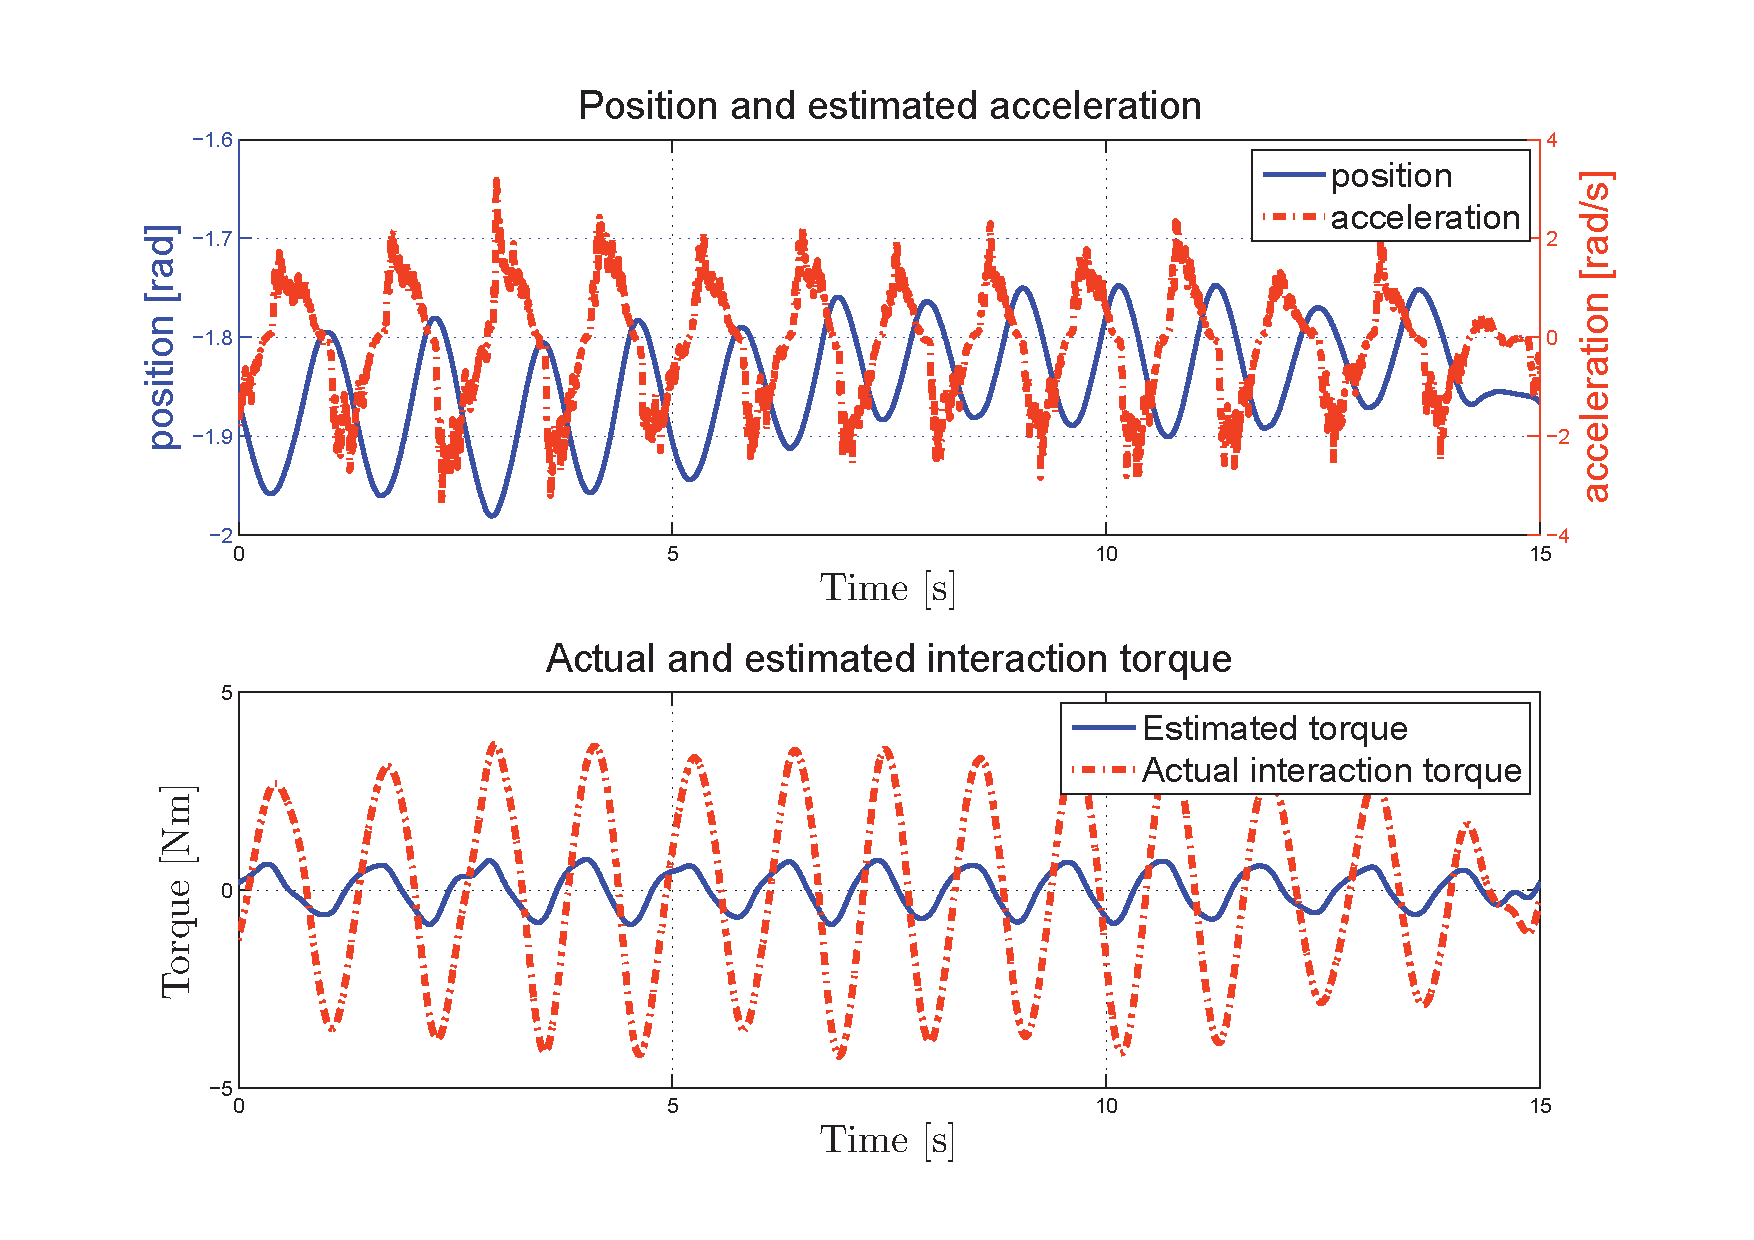
\includegraphics[width=1\columnwidth]{a_p_ts2_vs_ets2_nocomp.pdf}\label{fig:torque_validation_nocomp}}
	\subfigure[With dynamics compensation]{  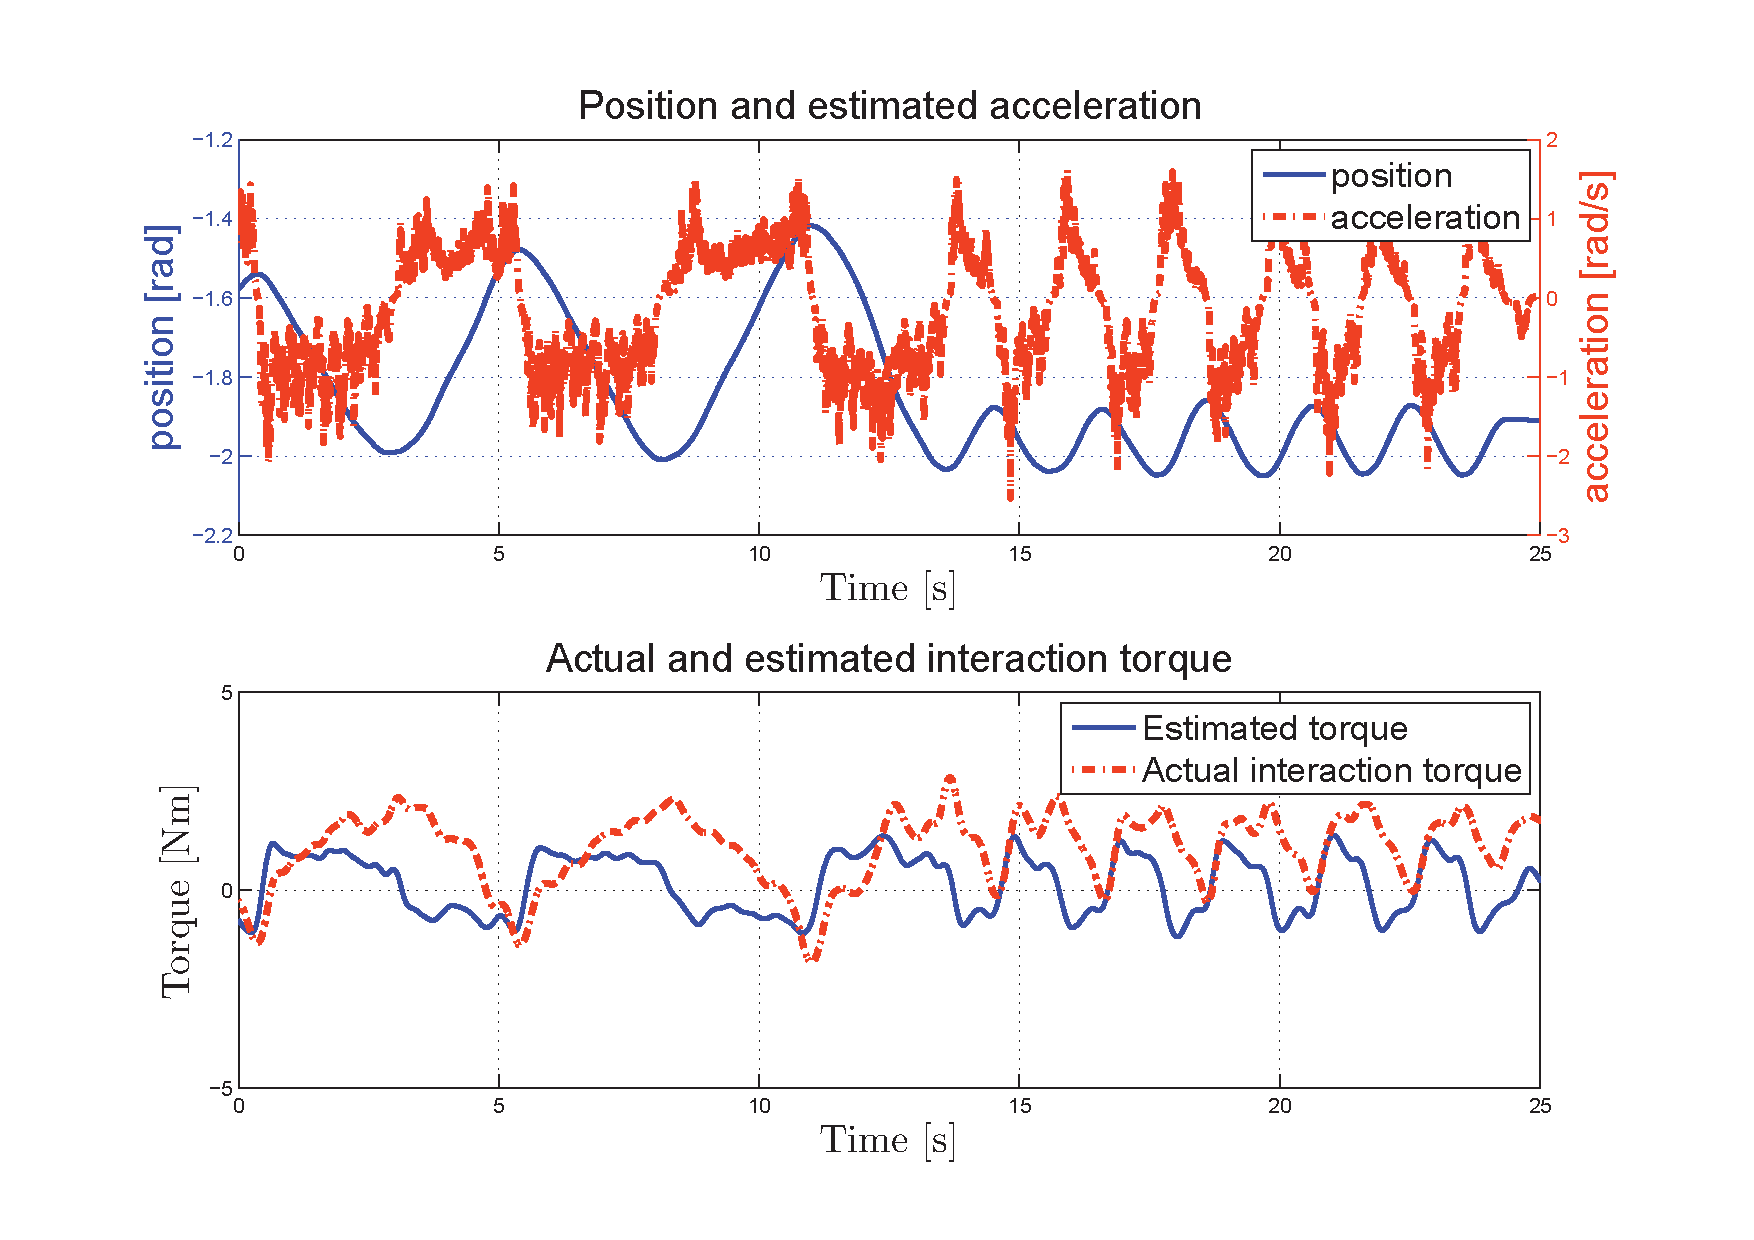
\includegraphics[width=1\columnwidth]{a_p_ts2_vs_ets2_comp.pdf}\label{fig:torque_validation_comp}}
	\caption{Comparison between the measured torque $\tau_s$ and calculated torque by force sensor}
	\label{fig:torque_validation}
\end{figure}



\subsubsection{Comparison between the three torque controllers JTFC1, JTFC2 and JTFC3}
For this kind of trials the three joint torque controls presented in the section \ref{sec:Full_state_feedback_controllers} were tested with a desired torque set to zero ($\vects{\tau_s^D=0}$) as for the trials in the subsection \ref{subsubsec:compensationAndTransparency}. 
\par In order to have comparable results and repeatability of trials, the transparency of the exoskeleton was tested with the same subject while he was trying to perform the same circular trajectory at the end effector, with the same velocity using the three different controls. The subject had visual cue (a circle of 150 mm of radius) while performing the task.
To evaluate the transparency performances only data in the same range of speed were used.
Despite the user tried to track the desired trajectory, the executed ones and their speeds were someway influenced by the used torque control. The average speed at the end effector of the three controls are listed in the \tablename \ \ref{tab:transparencySpeeds}.
%
%\begin{table}[!t]
%	\renewcommand{\arraystretch}{1.3}
%	\caption{The natural frequency of the joints}
%	\label{tab:transparencySpeeds}
%	\centering
%	\begin{tabular}{|c|c|c|}
%		\hline
%		\bfseries Control & \bfseries Avg. speed [$m/s$] & \bfseries Std. dev. [$m/s$]\\
%		\hline\hline
%		JTFC1 & 0.4198 & 0.0810\\
%		\hline
%		JTFC2 & 0.4460 & 0.1374\\
%		\hline
%		JTFC3 & 0.3867 & 0.1213\\
%		\hline
%	\end{tabular}
%\end{table}
\begin{table}[]
	\renewcommand{\arraystretch}{1.3}
	\caption{Mean and Std. Dev. of the e.e. speed in the transparency experiments}
	\label{tab:transparencySpeeds}
	\centering
	\begin{tabular}{c c c}
		\hline \hline
		\bfseries Control & \bfseries Avg. speed [$m/s$] & \bfseries Std. dev. [$m/s$]\\
		\hline
		JTFC1 & 0.4198 & 0.0810\\
		JTFC2 & 0.4460 & 0.1374\\
		JTFC3 & 0.3867 & 0.1213\\
		\hline \hline
	\end{tabular}
\end{table}
%
The real trajectories can be shown in the \figurename \ \ref{fig:traittorie3D}.
\begin{figure}[htb]
	\centering
	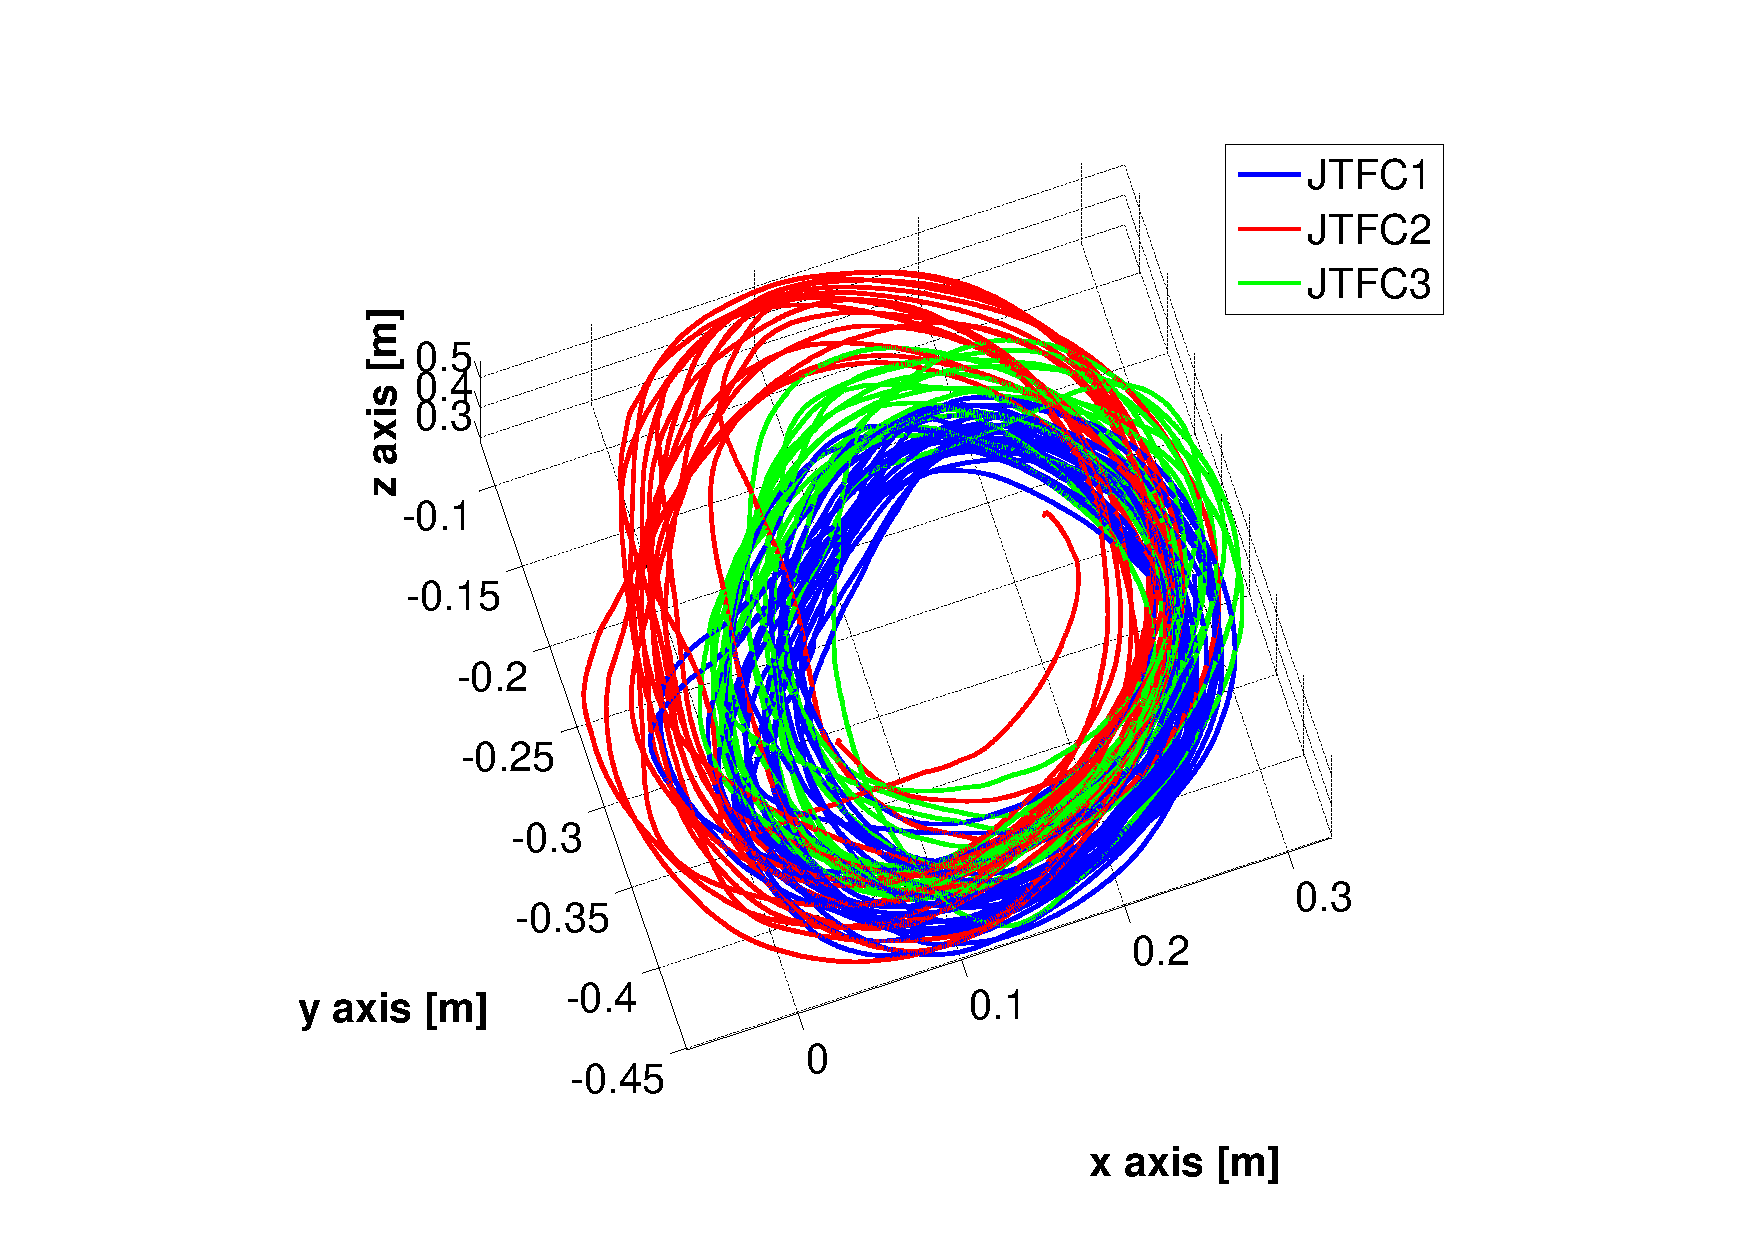
\includegraphics[width=0.99\columnwidth]{traiettorieCircolari2}
	\caption{The trajectories performed during the transparency test using the three control laws.}
	\label{fig:traittorie3D}
\end{figure}
%\begin{figure}[htb]	
%	\centering
%	\includegraphics[width=0.7\columnwidth]{\figpath{traiettorieCircolariPianoXY}}
%	\label{fig:traiettorieXY}
%	\caption{The Rehab-Exos CAD model showing overall kinematics and actuator structure}
%\end{figure}
%
\par As the reader can see, the red trajectories (the ones obtained by using the control JTFC2) are less accurate due to the limited torque control performance. Moreover, from the analysis of the control torque errors at the joints (\figurename \ \ref{fig:transparencyJointErrors}), it can be seen that the control JTFC2 exhibits an average error that is independent from the link inertia. The torque error over link inertia ratio for the elbow joint is the highest and this leads to a greater disturbance on the fine trajectory execution.
\begin{figure}[htb]
	\centering
	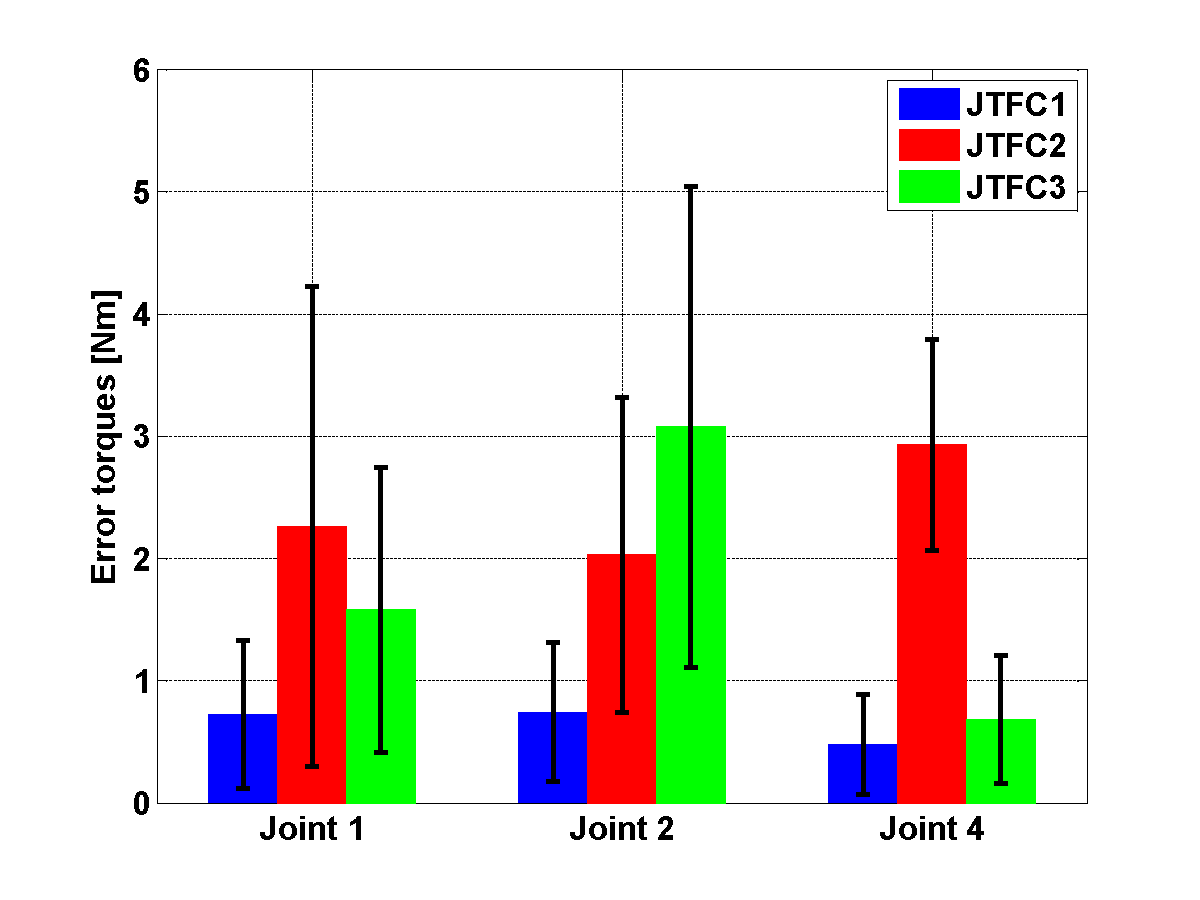
\includegraphics[width=1\columnwidth]{erroriTrasparenzaGiunti}
	\caption{The torque errors of the 3 controllers for joints 1, 2 and 4.}
	\label{fig:transparencyJointErrors}
\end{figure}
%
The average force measured at the end effector are shown in \figurename \ \ref{fig:transparencyEeErrors}.
\begin{figure}[htb]
	\centering
	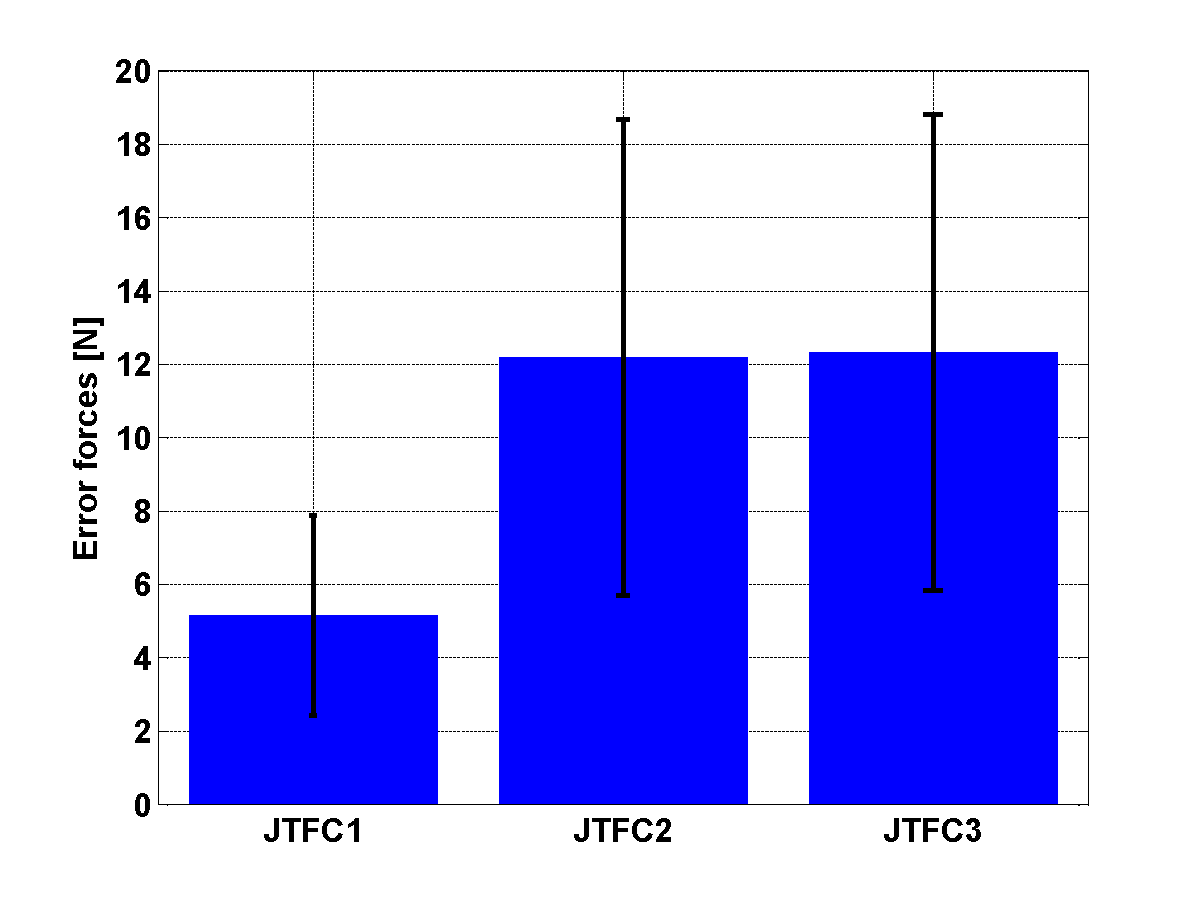
\includegraphics[width=1\columnwidth]{erroreForzaEETrasparenza}
	\caption{The force error at the end effector of the 3 controllers.}
	\label{fig:transparencyEeErrors}
\end{figure}
%
\par The value of the end-effector forces provides an overall index of the exoskeleton transparency with a given torque control (when $\vects{\tau_s^D=0}$). The control JTFC1 that implements a full-state feedback control performs better because it models in a more accurate and general way the joint dynamics. Moreover, the control JTFC1 compensates for the modeled effects. Notice that, at joint level, the control JTFC3 behaves more similar to JTFC1 rather than to the control JTFC2, in fact the torque errors of the control JTFC1 and JTFC3 seems to be correlated to the link inertia.

%%%%%%%%%%%%%%%%%%%%%%%%%%%%%%%%%%%%%%%%%%%%%%%%%%%%%%%%%%%%%%%%%%%%%%%%%%%%%%%%%%%%%%%%%%%%%%%%%%%%%%%%%%%%%%%%%%%%
%%%%%%%%%%%%%%%%%%%%%%%%%%%%%%%%%%%%%%%%%%%%%%%%%%%%%%%%%%%%%%%%%%%%%%%%%%%%%%%%%%%%%%%%%%%%%%%%%%%%%%%%%%%%%%%%%%%%
\subsection{Haptic rendering}

The implemented torque controls can be used to render the interaction forces exchanged with a virtual surface of a given stiffness and damping, acting as impedance controls. In these tests the contact forces at the end-effector are proportional to the penetration length of the end-effector into the virtual wall surface and to its speed. The force is then converted to desired torques at the joints by multiplying the equation defined in (\ref{eq:desiredVE}) by the transpose of the Jacobian, where the equations (\ref{eq:JTCF1_control_law_uf_simple}), (\ref{JTFC2_control_law_final}) and (\ref{control_law_Kugi_2}) have been used respectively for JFTC1, JFTC2 and JFTC3.
%The design of the exoskeleton allows to control the torque on every joint, so it is possible to render an interaction force not only at the end effector but on every link of the robot. In this case, in equation (\ref{jacobian}) a modified Jacobian will be used to convert forces not applied on the end effector.
\par In the experiments the user grabs the exoskeleton only at the end effector without applying any other force on the links. In this way, the forces measured by the end-effector's force sensor have been used to evaluate the overall system performance since these forces are not involved for the torque control.
\par The rendering experiments were composed by four different type of trials as depicted in \figurename \ \ref{fig:renderingTestType}:
\begin{itemize}
	\item T1: "Slide on surface" experiment with moderate forces;
	\item T2: "Slide on surface" experiment with high forces;
	\item T3: "Collision with a surface" experiment with moderate speed;
	\item T4: "Collision with a surface" experiment with high speed.
\end{itemize}

During the T1 and T2 trials the experimenter slided the end-effector on the surface without sudden variations of penetration. The difference between the T1 and T2 trials is the average level of force along the orthogonal axes at the surface.
In the T3 and T4 trials the aim is to test the dynamic performance of the controls, so the experimenter pushed the end-effector on the surface. The difference between the T3 and T4 trials is the average slope of the desired force profiles.
The 4 tests have been evaluated for each controls and with three different environment parameters, in order to consider a low, an intermediate and a high stiff wall. 
\begin{figure}[htb]
	\centering
	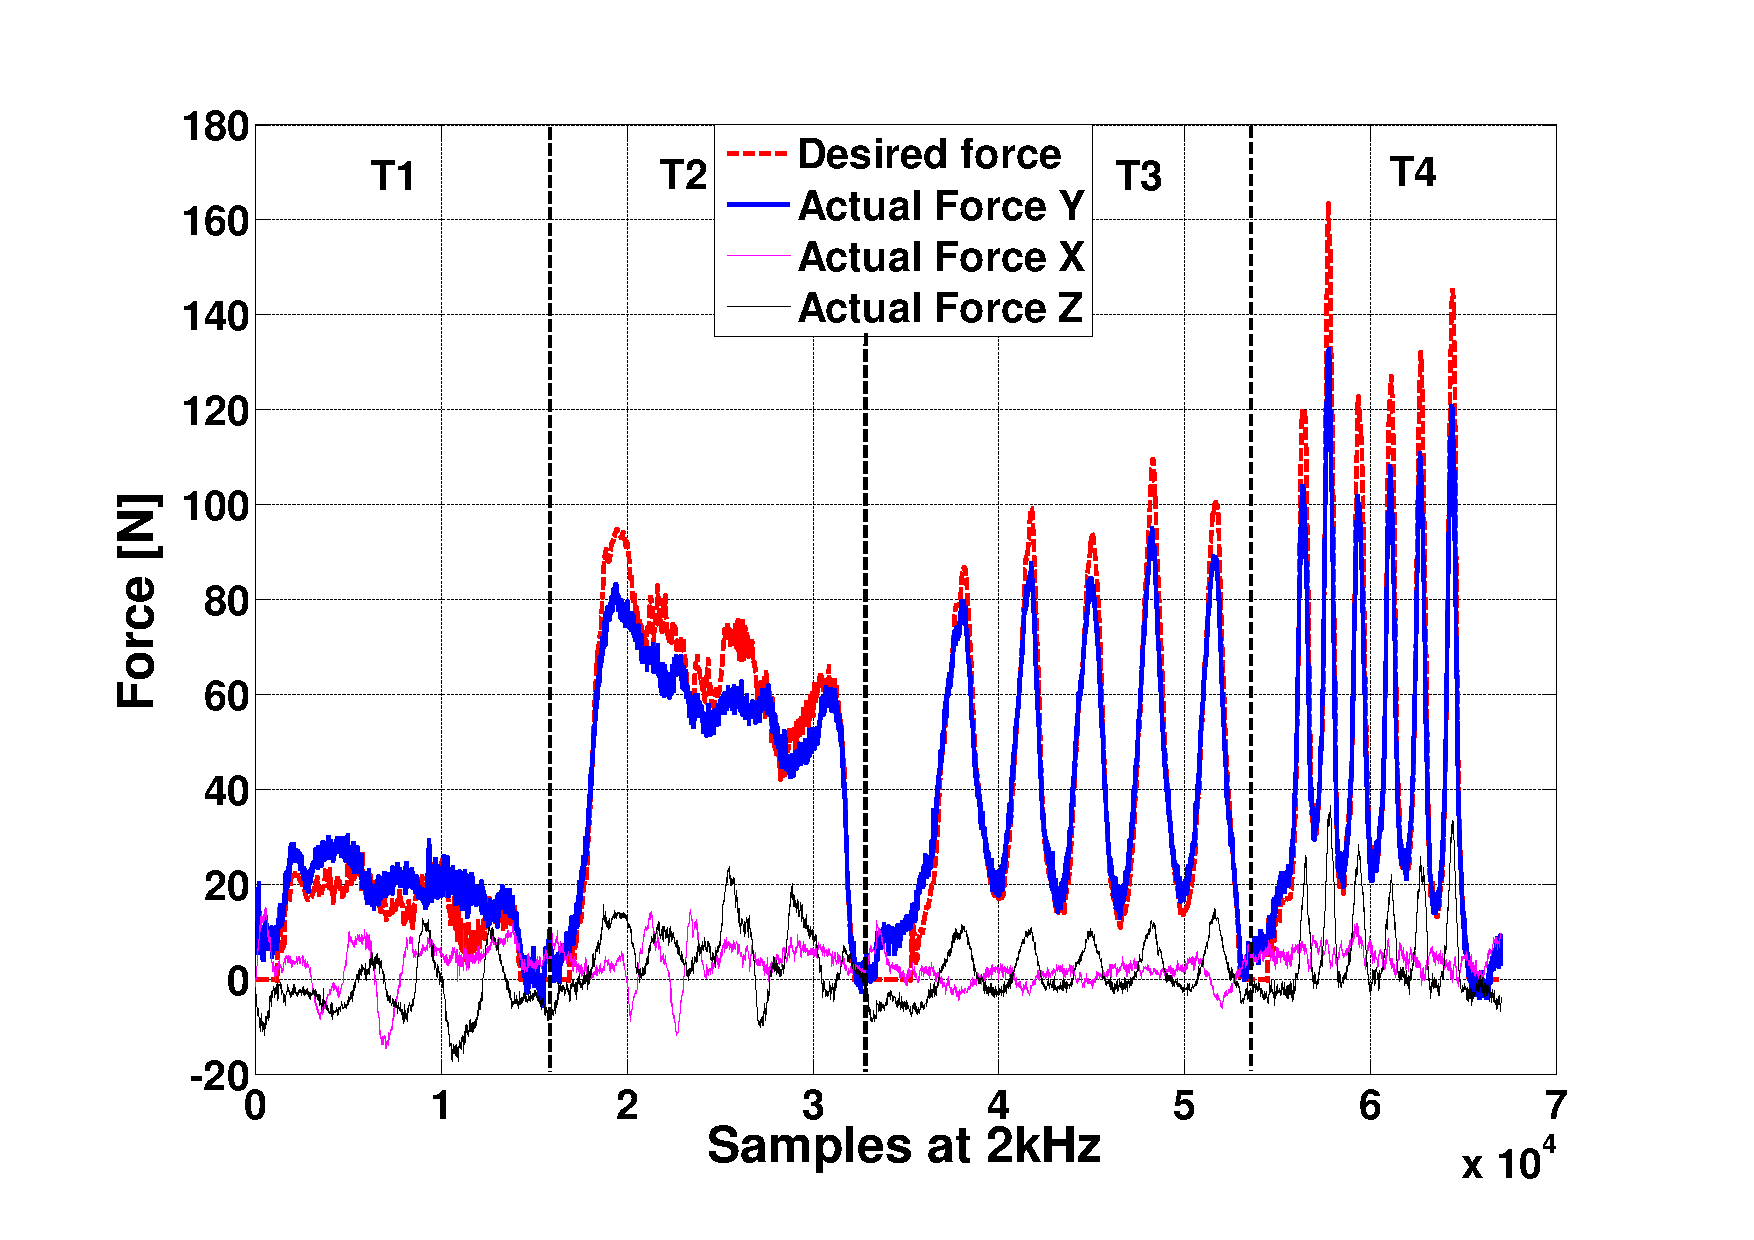
\includegraphics[width=1\columnwidth]{proveRendering}
	\caption{The four trial types during an haptic rendering test. The desired forces is plotted with red dashed lines, the measured orthogonal forces are plotted with blue solid lines while the two tangential components are with magenta and black solid lines.}
	\label{fig:renderingTestType}
\end{figure}

\par The \tablename \ \ref{tab:meanForcesRendering} reports the three environment parameters, the average forces involved in the T1 and T2 trials, the average force peaks and the average slope of the T3 and T4 trials.
%\begin{table}[!t]
%	\renewcommand{\arraystretch}{1.3}
%	\caption{The average forces involved in the T1 and T2 trials, the average force peaks and the average slope of the T3 and T4 trials.}
%	\label{tab:meanForcesRendering}
%	\centering
%	\begin{tabular}{|c|c|c|c|c|}
%		\hline
%		\bfseries Env. Params. & \bfseries T1 & \bfseries T2 & \bfseries T3 & \bfseries T4 \\
%		\hline\hline
%		5 kN/m  &  22.22 $N$ & 50.79 $N$ & 83.33 $N$ & 112.33 $N$\\ 2 Ns/m & - & - & 127.28 $N/s$ & 518.49 $N/s$\\ 
%		\hline
%		20 kN/m &  22.81 $N$ & 66.14 $N$ & 103.97 $N$ & 136.97 $N$\\ 7 Ns/m & - & - & 159.25 $N/s$ & 550.99 $N/s$\\
%		\hline
%		40 kN/m  &  24.98 $N$ & 59.37 $N$ & 88.32 $N$ & 126.20 $N$\\ 10 Ns/m & - & - & 120.39 $N/s$ & 616.03 $N/s$\\
%		\hline
%	\end{tabular}
%\end{table}
\begin{table}[]
	\renewcommand{\arraystretch}{1.3}
	\caption{The average forces involved in the T1 and T2 trials, the average force peaks and the average slope of the T3 and T4 trials.}
	\label{tab:meanForcesRendering}
	\centering
	\begin{tabular}{c c c c c}
		\hline \hline
		\bfseries Env. Params. & \bfseries T1 & \bfseries T2 & \bfseries T3 & \bfseries T4 \\
		\hline
		5 kN/m  &  22.22 $N$ & 50.79 $N$ & 83.33 $N$ & 112.33 $N$\\ 2 Ns/m & - & - & 127.28 $N/s$ & 518.49 $N/s$\\ 
		\hline
		20 kN/m &  22.81 $N$ & 66.14 $N$ & 103.97 $N$ & 136.97 $N$\\ 7 Ns/m & - & - & 159.25 $N/s$ & 550.99 $N/s$\\
		\hline
		40 kN/m  &  24.98 $N$ & 59.37 $N$ & 88.32 $N$ & 126.20 $N$\\ 10 Ns/m & - & - & 120.39 $N/s$ & 616.03 $N/s$\\
		\hline \hline
	\end{tabular}
\end{table}

\par To evaluate the performances of the three different torque controls three indexes have been proposed, i.e. 
\begin{itemize}
	\item the mean of the norm of the error force vectors;
	\item the mean of the absolute value of the error of the orthogonal component;
	\item the mean of the angle between the desired forces and the measured ones.
\end{itemize}

\begin{figure}[htb]
	\centering
	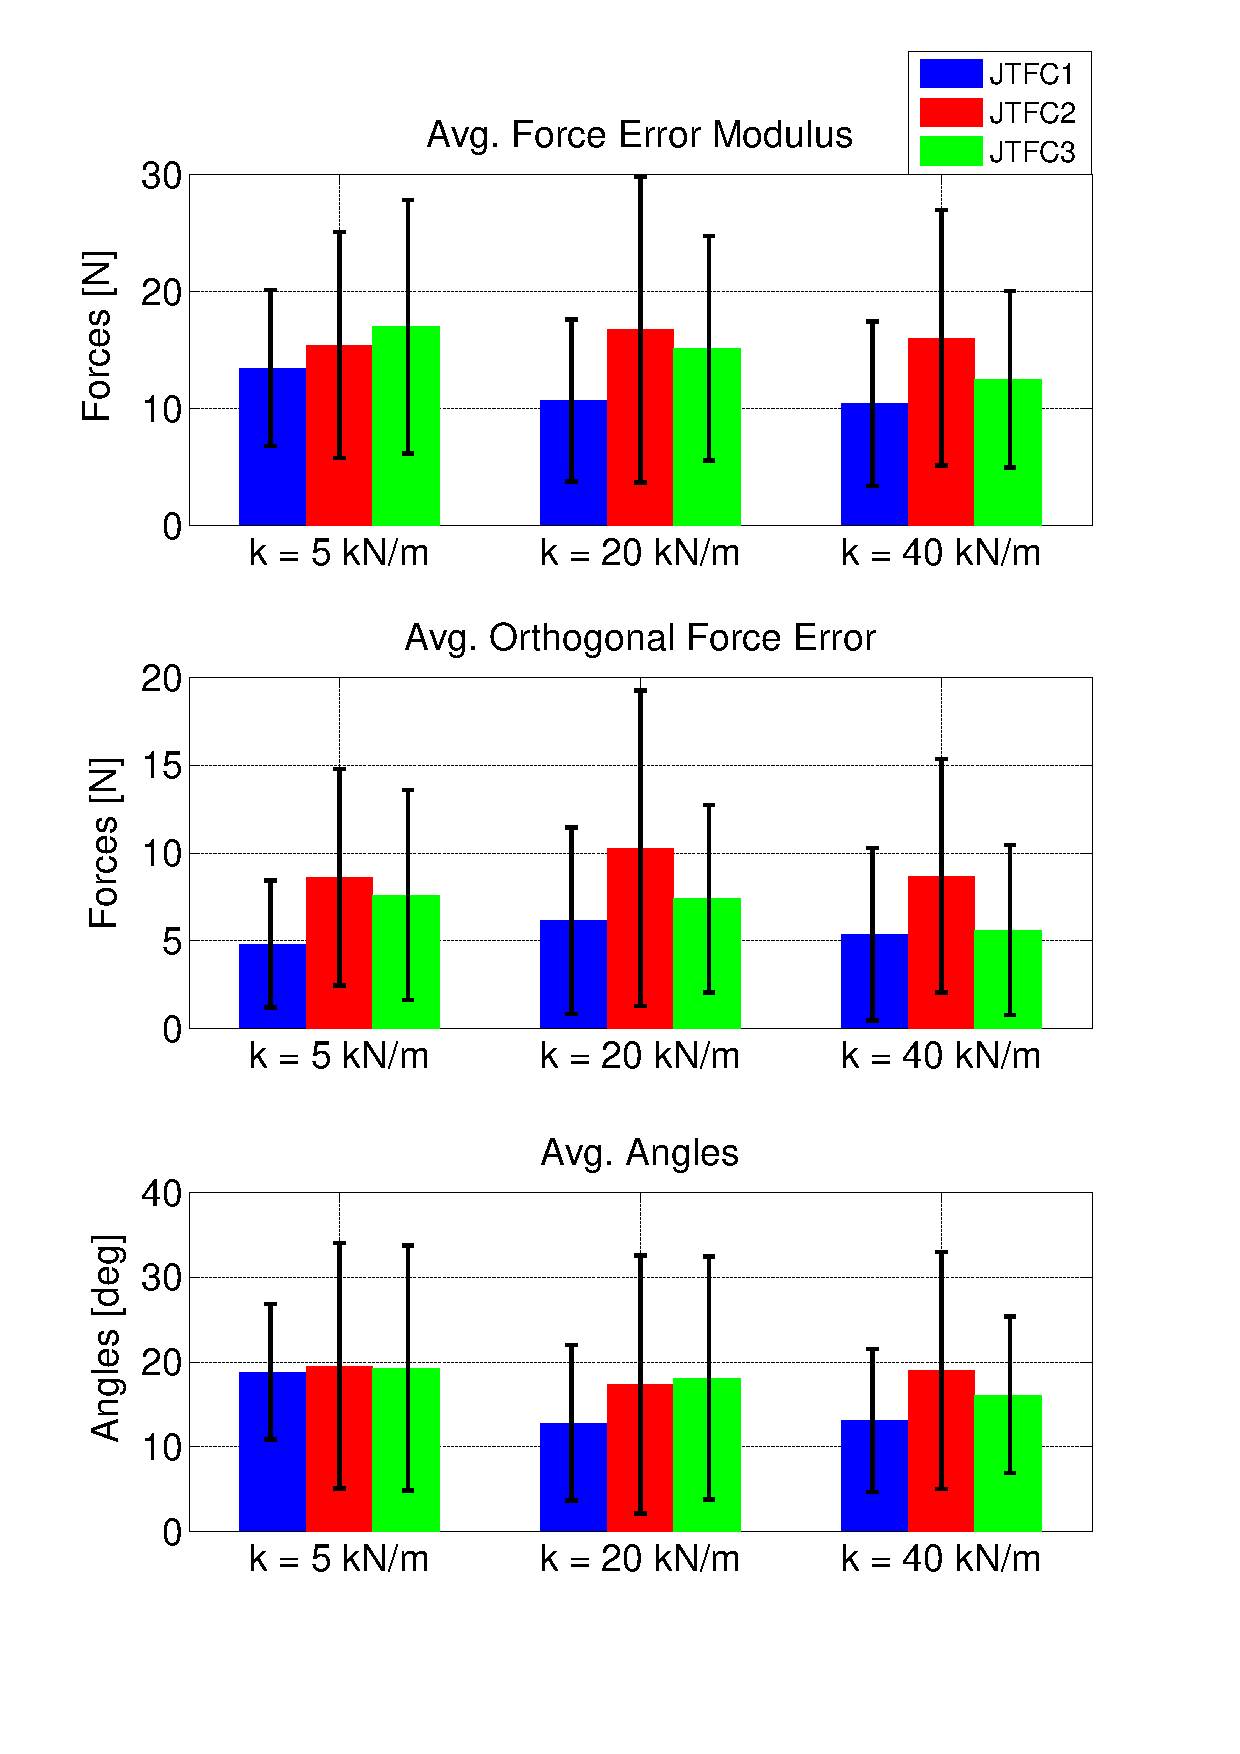
\includegraphics[width=1\columnwidth]{erroriForzeAngoliRendering}
	\caption{At the top, the average of the modulus of the error force vectors at the end effector of the 3 controllers in the rendering task. For this test, 3 stiffness has been evaluated: 5kN/m (small), 20 kN/m (medium) and 40 kN/m (high). In the middle, the average error forces of the orthogonal component. At the bottom, the average angle between the desired force vectors and the measured ones.}
	\label{fig:renderingErrors}
\end{figure}

\par The results can be shown in the \figurename \ \ref{fig:renderingErrors}. The first graph shows the average difference between the rendered forces by the controls and the desired forces with an aggregate index, i.e. the norm of the error vector. From this graph the reader can see that in all the condition the JTFC1 control performs better then the others, in fact the mean of the error is around 10 N in all the three cases.
\par To decompose the informations given in the first graph, other two indexes are considered, that are the average error of the orthogonal component of the force and the angle between the desired and the rendered forces. Unlike the norm of the error vector, these two indexes give information on the amplitude and the direction of the undesired force components. The second graph highlights that the JTFC1 control leads to an average error of 5 N along the task direction independently from the environment parameters, that is a good result coupled with the exhibited stable contact with the surface in every condition.
The third graph is substantially in agreement with the previous ones.

%%%%%%%%%%%%%%%%%%%%%%%%%%%%%%%%%%%%%%%%%%%%%%%%%%%%%%%%%%%%%%%%%%%%%%%%%%%%%%%%%%%%%%%%%%%%%%%%%%%%%%%%%%%%%%%%%%%%
%%%%%%%%%%%%%%%%%%%%%%%%%%%%%%%%%%%%%%%%%%%%%%%%%%%%%%%%%%%%%%%%%%%%%%%%%%%%%%%%%%%%%%%%%%%%%%%%%%%%%%%%%%%%%%%%%%%%
%%%%%%%%%%%%%%%%%%%%%%%%%%%%%%%%%%%%%%%%%%%%%%%%%%%%%%%%%%%%%%%%%%%%%%%%%%%%%%%%%%%%%%%%%%%%%%%%%%%%%%%%%%%%%%%%%%%%
%%%%%%%%%%%%%%%%%%%